\section{Lernfeld 2 - Geschäftsprozesse und betriebliche Organisation}

%%% Anfang: tl;dr
\subsection{tl;dr - Zusammenfassung der Zusammenfassung}
%%% Ende: tl;dr
%%%%%%%%%%%%%%%%%%%%%%%%%%%%%%%%%%%%%%%%%%%%%%%%%%%%%%%%%%%%%%%%%%%%%%%%%%%%%%%%

%%% Anfang: Projektmanagment
\subsection{Projektmanagment}

%%% Anfang: Projektmanagment > Kriterien
\subsubsection{Kriterien eines Projektes}
\begin{itemize}
	\item Einmaligkeit
	\item Zeitbegrenzung
	\item Bedeutsamkeit
	\item Komplexität
	\item Fachübergreifend
	\item Risiko
\end{itemize}

%%% Anfang: Projektmanagment > Anlässe
\subsubsection{Anlässe für Projekte}
\begin{itemize}
	\item Organisatorische Probleme: schlechter Informationsfluss
	\item Technische Probleme: hoher Wartungsaufwand
	\item Wirtschaftliche Probleme: sinkende Umsätze
	\item Marktbezogene Entwicklungen: Wettbewerbsdruck
	\item Innovation: neue Produktideen
	\item Controlling-Ergebnisse: ineffiziente Systeme
\end{itemize}

%%% Anfang: Projektmanagment > Dreieck
\subsubsection{Magisches Dreieck des Projektmanagments}

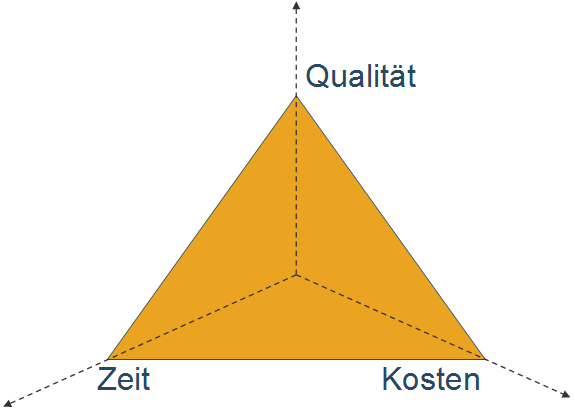
\includegraphics[scale=0.4]{pictures/lf02-pic/lf02-projekt-dreieck.png}

Zeit und Kosten lassen sich quantitativ relativ einfach festlegen, auch der Leistungsumfang. Schwierig wird es bei der Festlegung der Qualität. Ein Projektergebnis hat nicht \ql eine\qr\ Qualität, sondern verschiedene Qualitätsmerkmale, wie z.B. Fehlerfreiheit, Robustheit, Zuverlässigkeit, Lebensdauer und Funktionalität.

%%% Anfang: Projektmanagment > Planungsphasen
\subsubsection{Planungsphasen von Projekten}
\begin{enumerate}
	\item Definition
	\begin{enumerate}
		\item Die im Projekt-Auftrag formulierten Ziele werden in einer dem Fachgebiet entsprechenden und auf die Durchführung ausgerichteten Terminologie beschrieben.
		\item Wenn noch kein Lastenheft vom Projekt-Kunden erstellt wurde, gehört auch die Präzisierung und Ausformulierung der Projektziele in diese Phase.
	\end{enumerate}
	\item Analyse
	\begin{enumerate}
		\item Das Projektziel wird in Teilziele zerlegt und daraus werden sogenannte Arbeitspakete abgeleitet.
		\item Arbeitspakete werden in einem Projektstrukturplan dargestellt, die Arbeitspaket-Definitionen verschriftlicht und im sogenannten Pflichtenheft vertraglich zugesichert.
	\end{enumerate}
	\item Realisierungsplanung
	\begin{enumerate}
		\item Antworten auf folgende W-Fragen müssen gefunden werden:
			\begin{enumerate}
				\item {\bf Was} soll mit dem Projekt bzw. in einem Projektabschnitt {\it tatsächlich} realisiert werden, bzw. was ist zunächst {\it nicht} machbar? Hilfsmittel sind z.B. Machbarkeits-/Durchführbarkeitsanalysen, Nutzwert- und Kosten-Nutzenanalysen etc.
				\item {\bf Wie} bzw. {\bf wie gut} soll die Realisierung erfolgen (Qualitätsziel)?
				\item {\bf Wie viel} soll realisiert werden (Quantitätsziel)
				\item {\bf Wer} soll (bestimmte Aufgaben) realisieren (Personalressourcen)?
				\item {\bf Womit} bzw. {\bf wodurch} soll die Realisierung erfolgen (Einsatz von Material-Ressourcen, Budget, \dots)?
				\item {\bf Wann} bzw. {\bf wie lange} soll/darf die Realisierung erfolgen?
				\item {\bf Wo} soll die Realisierung erfolgen (Standort)?
			\end{enumerate}				 
		\item Die Ergebnisse dieser letzten Phase sind Tätigkeitslisten, Funktions- u. Verantwortungsmatrix, Terminliste, Balkendiagramme, Netzpläne, Meilensteinlisten, Kosten- und Finanzpläne usw.
	\end{enumerate}	
\end{enumerate}

%%% Anfang: Projektmanagment > Projektantrag/-auftrag
\subsubsection{Projektantrag und Projektauftrag}

Ein Projektantrag stellt nach DIN 69905 ein \ql Antrag auf Projektgründung\qr\ dar. Stellung ist typisch für interne Projekte oder öffentlich geförderte Projekte. Wenn ein \textbf{Projektantrag} genehmigt wird, wird daraus ein \textbf{Projektauftrag}. Der Projektantrag enthält folgende Informationen:
\begin{itemize}
	\item Aufgabenbeschreibung
	\item Erwarteter Nutzen
	\item Konsequenzen bei Nicht-Beachtung
	\item Rahmenbedingungen
\end{itemize}
\noindent Durch einen Projektauftrag werden die Verbindlichkeiten für beide Seite geregelt. Im Detail werden die folgenden Punkte schriftlich fixiert:
\begin{itemize}
	\item Was soll realisiert werden?
	\item Welche Qualität wird angestrebt?
	\item Wie viel soll realisiert werden?
	\item Personal: wer wird eingesetzt?
	\item Material: womit wird die Realisierung erfolgen?
	\item Zeitrahmen: wie lange soll das Projekt dauern?
	\item Wo soll das Projekt umgesetzt werden?
	\item Welche Risiken bestehen?
\end{itemize}

%%% Anfang: Projektmanagment > Lasten-/Pflichtenheft
\subsubsection{Lasten- und Pflichtenheft}

\begin{tabular}{ | p{\dimexpr 0.5\linewidth-2\tabcolsep} |
p{\dimexpr 0.5\linewidth-2\tabcolsep} | }
		\hline
		{\bf Lastenheft} & {\bf Pflichtenheft}\\
		\hline
		Anforderungsspezifikationen & Sollkonzept\\
		Grobes Pflichtenheft & Fachfeinkonzept\\
		& Fachliche Spezifikation\\
		\hline
		Beschreibt die unmittelbaren Anforderungen und Wünsche an ein geplantes Projekt & Ist die vertraglich bindende,detaillierte Beschreibung einer zu erfüllenden Leistung, zum Beispiel dem Aufbau einer technischen Anlage, der Konstruktion eines Werkzeugs oder auch der Erstellung eines Computerprogramms\\
		\hline
		vom Auftraggeber festgelegte Gesamtheit der Forderungen an die Lieferungen und Leistungen eines Auftragnehmers innerhalb eines Auftrages & vom Auftragnehmer erarbeitete Realisierungsvorhaben aufgrund der Umsetzung des vom Auftraggeber vorgegebenen Lastenhefts\\
		\hline
		Was und Wofür & Wie und Womit\\
		\hline
		Die Adressaten des Lastenhefts sind der (externe oder firmeninterne) Auftraggeber, sowie die Auftragnehmer &\\
		\hline
		In der Softwaretechnik ist das Lastenheft das Ergebnis der Planungsphase und wird in der Regel von den Entwicklern als Vorstufe des Pflichtenhefts erarbeitet & Die Inhalte des zuvor ausgearbeiteten Lastenhefts sind nun präzisiert, vollständig und nachvollziehbar sowie mit technischen Festlegungen der Betriebs- und Wartungsumgebung verknüpft\\
		\hline
\end{tabular}\newline

Gewöhnlich können jeder Anforderung des Lastenhefts eine oder mehrere Leistungen des Pflichtenhefts zugeordnet werden. So wird auch die Reihenfolge der beiden Dokumente im Entwicklungsprozess deutlich: Die Anforderungen (requirements) werden durch Leistungen (features) erfüllt.\newline

\paragraph{Pflichtenheft (Aufbau nach Balzert)}~\\
\begin{itemize}
	\item Zielbestimmung: Die Ziele des Produktes sind in drei Kategorien geordnet
	\begin{itemize}
		\item Musskriterien: was ist notwendig?
		\item Wunschkriterien: was ist gefordert?
		\item Abgrenzungskriterien: was wird nicht gefordert?
	\end{itemize}
	\item Produkteinsatz
	\begin{itemize}
		\item Umfeld der Anwendung
		\item Benennung des späteren Anwendungsbreiches, der Zielgruppe und der Betriebsbedingungen
	\end{itemize}
	\item Produktübersicht
	\begin{itemize}
		\item Übersicht über alle die Anwendung betreffende Geschäftsprozesse
	\end{itemize}
	\item Produktfunktion
	\begin{itemize}
		\item Unterstützte Produktfunktionen (Anwendungsfall, Bedingungen, Auswirkungen)
	\end{itemize}
	\item Produktdaten
	\begin{itemize}
		\item Produktleistung (bestimmte Leistungsanforderungen? Sind diese erfüllbar?)
		\item Qualitätsanforderungen (Funktionalität, Zuverlässigkeit, Benutzbarkeit, Effizienz, Änderbarkeit und Übertragbarkeit)
		\item Benutzungsoberfläche (grundlegende Anforderungen, Zugriffsrechte)
		\item Nichtfunktionale Anforderungen (nicht die Funktion der Software betreffend, bspw. rechtliche Vorgaben)
		\item Anforderungen an die Entwicklungsumgebung (notwendige Hardware, Software)
		\item Gliederung in Teilpunkte (Teilpunkte des Projektes und deren Funktionalität)
		\item Ergänzungen (Anforderungen, die vorher keinen Platz hatten)
		\item Globale Testfälle (wichtigste Testfälle, größten Teil der Funktionen abdecken)
	\end{itemize}
\end{itemize}

%%% Anfang: Projektmanagment > Bedeutung
\subsubsection{Warum hat Projektmanagement an Bedeutung gewonnen?}
\begin{itemize}
	\itemsep0em
	\item Fachübergreifende Aufgaben nehmen zu
	\item Immer mehr hin zu einmaligen und speziellen Aufgaben
	\item Sicherung von Qualität
	\item Unternehmen müssen stärkerem Konkurrenzdruck standhalten; Wirtschaftlichkeit
	\item Kundenorientiertes Arbeiten
	\item Einhalten von konkreten Zeitplänen
\end{itemize}

%%% Anfang: Projektmanagment > Organisation
\subsubsection{Projektorganisation}

Einsatzgebiet

\begin{itemize}
	\item Am häufigsten angewendete Projektform in Unternehmen
	\item Mitarbeiter gehen ihrer täglichen Arbeit nach
	\item Oberstes Ziel ist die Vernetzung von Ressourcen und deren optimaler Einsatz
	\item Mehrere Projekte können durch die Organisation mit den zusammengeführten Stellen und dem Projektleiter nebeneinander bearbeitet und erfolgreich abgeschlossen werden
	\item Mitarbeiter müssen am Ende des Projektes nicht um ihren Arbeitsplatz bangen
\end{itemize}

\noindent Reine Projektorganisation

\begin{itemize}
	\item Einrichtung einer eigenen und selbstständigen Organisationseinheit
	\item Projektmitglieder werden aus den Fachabteilungen abgezogen (oder extern beschafft) und einem Projektleiter unterstellt
	\item Projektleiter trägt im Idealfall allein die Verantwortung für das Erreichen der Projektziele und hat dem entsprechende umfangreiche Befugnisse
	\begin{itemize}
		\item Entscheidung mit der Unternehmensleitung über die Auswahl der Mitarbeiter und die Verteilung des Budgets
		\item Weisungsbefugnis gegenüber allen Mitarbeitern
		\item Anspruch auf alle projektrelevanten Informationen
		\item Letzte Entscheidung liegt im Zweifelsfall bei ihm
		\item Hohe Anforderungen in fachlicher, methodischer sowie sozialer Hinsicht
	\end{itemize}
	\item Konkurrenz der bearbeiteten Projekte untereinander: \ql Kampf der Projektleiter um Ressourcen\qr\
\end{itemize}

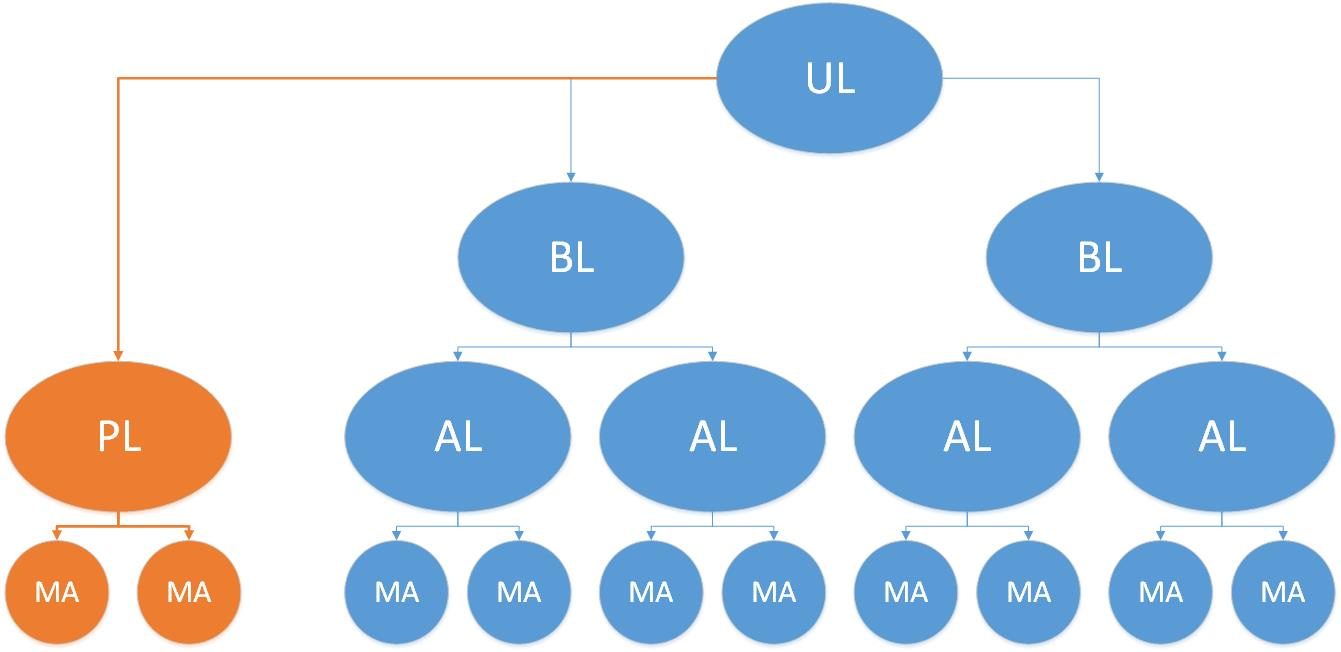
\includegraphics[scale=0.3]{pictures/lf02-pic/lf02-reine-projektorganisation.jpg}

%%% Anfang: Projektmanagment > Koordination
\subsubsection{Projektkoordination}
\begin{itemize}
	\item Statt eines Projektleiters gibt es einen Projektkoordinator mit beratender Funktion
	\begin{itemize}
		\item Koordiniert die Mitarbeit der Projektmitglieder
		\item Keine Entscheidungs- und Weisungsbefugnis im Rahmen des Projekts
	\end{itemize}
	\item Arbeit wird aus den verschiedenen Fachabteilungen erledigt
\end{itemize}

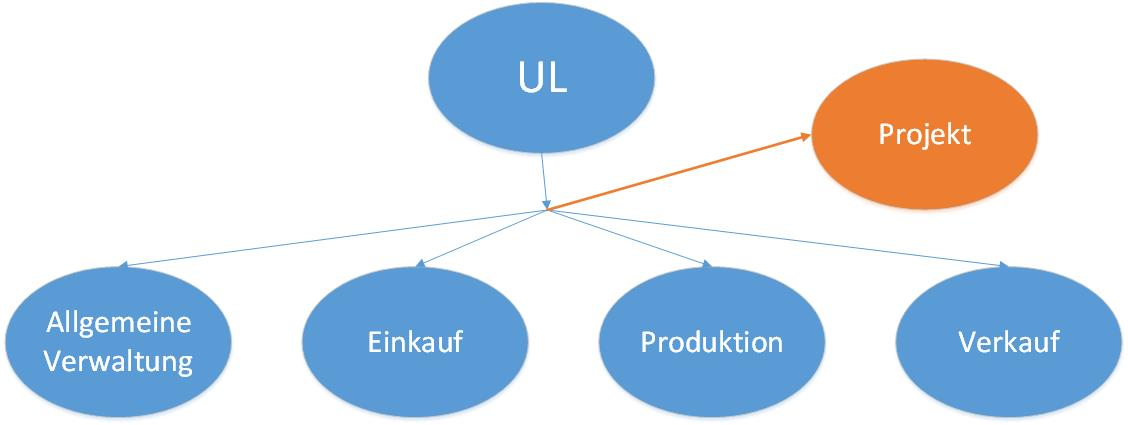
\includegraphics[scale=0.3]{pictures/lf02-pic/lf02-projektkoordination.jpg}

\paragraph{Matrixprojektorganisation}~\\
\begin{itemize}
	\item Alle beteiligten Mitarbeiter sind zwei Instanzen untergeordnet
	\begin{itemize}
		\item Linienverantwortliche
		\item Projektleiter hat die Verantwortung bezüglich des Projekts
	\end{itemize}
	\item Projektleiter obliegt die Verantwortung in der Abstimmung aller Projektbezogenen Aufgaben
	\item Linienverantwortlichen obliegt die fachliche Verantwortung
	\item Mitarbeiter gehen für gewöhnlich ihrer Basisarbeit nach und arbeiten einen gewissen Anteil ihrer Arbeitszeit für das Projekt
	\item Projektleiter wird ermöglicht, das Projekt rasch voranzutreiben, während die Linienverantwortlichen für einen optimalen Ressourceneinsatz und für eine adäquate Bearbeitung verantwortlich sind
	\item Verteilung der Aufgaben bzw. Verantwortungen ergeben Schnittstellen, die entsprechendes Konfliktpotential hervorrufen
	\begin{itemize}
		\item Meinungsverschiedenheiten entstehen
		\item Nur eine Einhaltung einer definierten Matrix Kultur und eine Kompromissbereitschaft kann im Interesse des Projektes zu gewünschten Erfolgen bzw. Ergebnissen führen
	\end{itemize}
\end{itemize}

%\includegraphics[scale=0.3]{pictures/lf02-pic/lf02-matrixorganisation.jpg}

%%% Ende: Projektmanagment
%%%%%%%%%%%%%%%%%%%%%%%%%%%%%%%%%%%%%%%%%%%%%%%%%%%%%%%%%%%%%%%%%%%%%%%%%%%%%%%%

%%% Anfang: Unternehmensorganisation
\subsection{Unternehmensorganisation}

[ An dieser Stelle sollte etwas stehen, dass die Grafik Einliniensystem und das Einliniensystem erklärt. ]

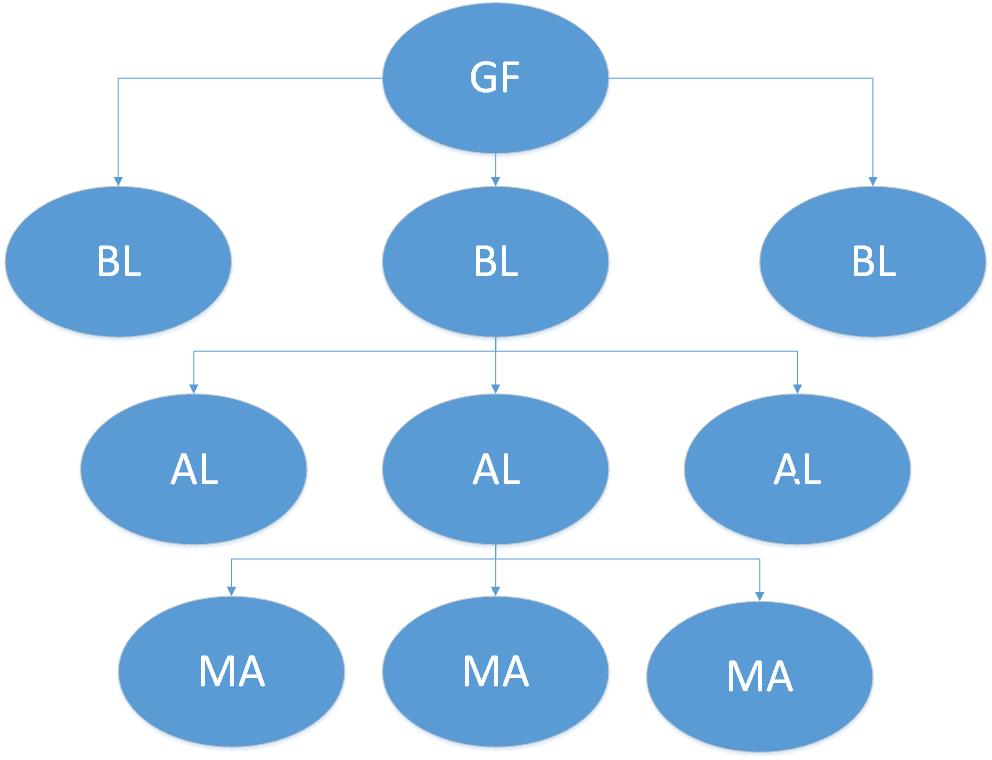
\includegraphics[scale=0.3]{pictures/lf02-pic/lf02-einliniensystem.jpg}

[ An dieser Stelle sollte etwas stehen, dass die Grafik Mehrliniensystem und das Mehrliniensystem erklärt. ]

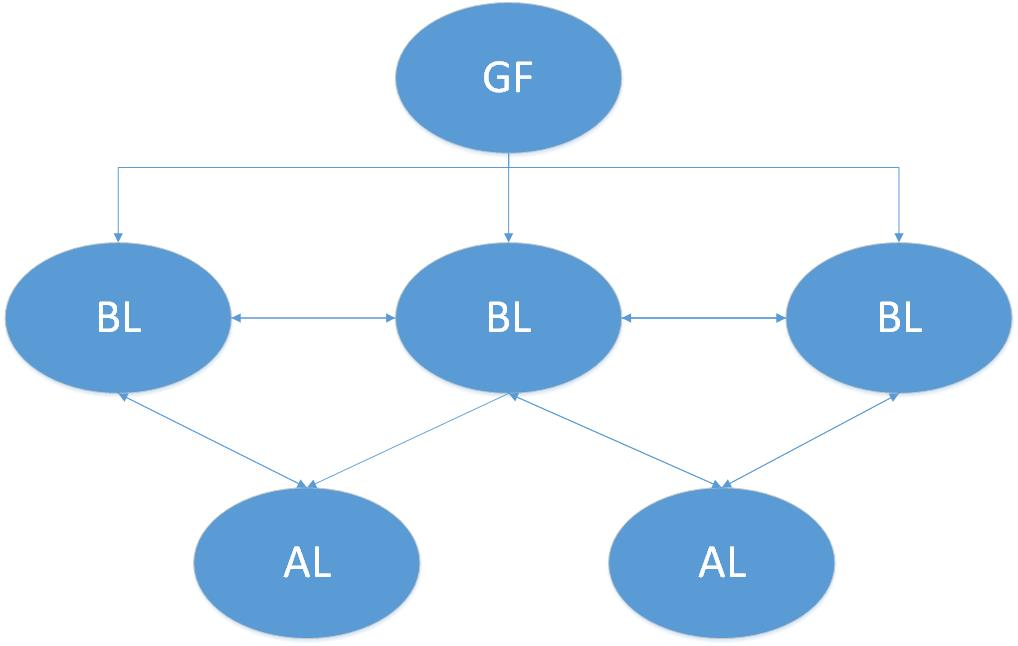
\includegraphics[scale=0.3]{pictures/lf02-pic/lf02-mehrliniensystem.jpg}

[ An dieser Stelle sollte etwas stehen, dass die Grafik Stabliniensystem und das Stabliniensystem erklärt. ]

\includegraphics[scale=0.3]{pictures/lf02-pic/lf02-stabliniensystem.jpg

%%% Ende: Unternehmensorganisation
%%%%%%%%%%%%%%%%%%%%%%%%%%%%%%%%%%%%%%%%%%%%%%%%%%%%%%%%%%%%%%%%%%%%%%%%%%%%%%%%

%%% Anfang: Projektcontrolling
\subsection{Projektcontrolling}

%%% Anfang: Projektcontrolling > Scorecard
\subsubsection{Balanced Scorecard}

%%% Ende: Projektcontrolling
%%%%%%%%%%%%%%%%%%%%%%%%%%%%%%%%%%%%%%%%%%%%%%%%%%%%%%%%%%%%%%%%%%%%%%%%%%%%%%%%

%%% Anfang: Mitarbeitermotivation
\subsection{Mitarbeitermotivation}
Motivation setzt sich aus drei Komponenten zusammen: (1) die Richtung, also was jemand erreichen will, (2) der Aufwand, den jemand bereit ist auf sich zu nehmen und (3) die Ausdauer, also wie lange jemand bereit ist diese Bemühungen aufrecht zu erhalten. Die Motivation bestimmt also die Richtung, Stärke und Dauer des menschlichen Handelns. Sie stellt die Energie dar, welche ein Individuum für eine bestimmte Handlung aufbringt.

Das Verhalten wird von einer Vielzahl von Motiven bestimmt, die abhängig sind von der Person und der Situation. Es wird zwischen primären und sekundären Motiven unterschieden. Bei primären Motiven handelt es sich um angeborene Motive wie beispielsweise Hunger. Sekundäre Motive sind abgeleitete Motive und durch die Struktur der Gesellschaft bestimmt. Sie können Ersatzmotive für primäre Motive darstellen, wie zum Beispiel der Wunsch nach Geld, mit dem sich dann Essen kaufen lässt. Sekundäre Motive werden durch Erfahrungen erlernt und sind sehr individuell.

Motiviert man einen Menschen in einem Unternehmen, dann möchte man den Mitarbeiter zu Handlungen veranlassen, die er grundsätzlich will (bzw. zumindest nicht ablehnt) und die im Sinne des Unternehmens sind.

Unterschied zur Manipulation: Bei der Manipulation wird der Mitarbeiter zu einem Verhalten beeinflusst, welches er eigentlich gar nicht will.
Motivation ist auf lange Zeit angelegt, Manipulation ist hingegen meist nur einmal oder für kurze Zeit wirksam.

Motivationsprozess
\begin{itemize}
	\item Mangel (Bedürfnis/Motiv) wird erfasst, wie z.B. das Bedürfnis nach Anerkennung. Die Umwelt gibt Anreize für die Beseitigung des Mangels
	\item Erfahrungswerte aus der Vergangenheit sind vorhanden, die erwarten lassen, dass der Mangel beseitigt werden kann (z.B. Erfahrungen mit der Erlangung von Anerkennung in einem anderen Unternehmen)
	\item Erkennen eines konkreten Weges, der zur Beseitigung des Mangels führt (z.B. verantwortliche Übernahme eines Projektes)
	\item Beschreiben des Weges, was zum Erfolg = Beseitigung des Mangels führen kann oder erfolglos bleibt
\end{itemize}

%%% Anfang: Mitarbeitermotivation > Herzberg
\subsubsection{Zweifaktortheorie nach Herzberg}

Untersuchungen sind primär auf die Frage nach der Zufriedenheit am Arbeitsplatz ausgerichtet. Die Mitarbeiter werden bei einer Verschlechterung der folgenden Grundfaktoren (Hygienefaktoren) unzufrieden:

\begin{itemize}
	\item Bezahlung
	\item Qualität der Personalführung
	\item Arbeitsbeziehungen zwischen Vorgesetzten, Kollegen und Untergebenen
	\item Arbeitsbedingungen
	\item Arbeitsplatzsicherheit
\end{itemize}

Verbesserungen dieser Faktoren wirken sich jedoch relativ neutral auf die Zufriedenheit aus. Die Hygienefaktoren sind die Rahmenbedingungen für die Leistungserstellung. Zufriedenheit lässt sich mit Motivatoren (Satisfaktoren) errreicht werden, die den Bedürfnissen entsprechen, welche aus der Arbeit selbst entstehen:

\begin{itemize}
	\item Leistung
	\item Anerkennung der Leistung durch andere
	\item Übertragung der Verantwortung
	\item Aufstiegschancen
	\item Entfaltungsmöglichkeiten
\end{itemize}

Zwei Feststellungen verdeutlichen die Nutzanwendung der Zweifaktorentheorie in der Personalführung: (1) Motivationspotenziale können durch mehrere Faktoren aktiviert werden und (2) den Hygienefaktoren kommt nicht der hohe motivationale Rang zu, wie lange Zeit angenommen.

Kritik an der Theorie besteht in erster Linie darin, dass sich Zufriedenheit nicht zuverlässig messen lässt. Dadurch ist nicht eindeutig nachvollziehbar, welche Faktoren zu der Zufriedenheit geführt haben. Des Weiteren können einige Faktoren für manche Personen lediglich ein Hygienefaktor sein, jedoch für andere Personen ein Motivator. Der Theorie kann zugutegehalten werden, dass sie gut praktisch anwendbar ist, wenn man der Theorie Glauben schenkt.

%%% Anfang: Mitarbeitermotivation > Maslow
\subsubsection{Bedürfnistheorie nach Maslow}

Maslow geht von fünf Bedürfniskategorien aus:
\begin{enumerate}
	\item Physiologische Bedürfnisse (Hunger, Schlafbedürfnis, Sexualität)
	\item Sicherheitsbedürfnisse beziehen sich auf die Gefahren, die dem Menschen aus seiner Umwelt erwachsen. Ordnung und Risikobegrenzung tragen zur Befriedigung der Sicherheitsbedürfnisse bei
	\item Soziale Beziehungen (soziale Kontakte, Zusammenleben in Gruppen)
	\item Anerkennung durch Dritte und Selbstachtung
	\item Selbstverwirklichung und Entfaltung
\end{enumerate}

Die ersten vier Bedürfnisse werden als {\it Defizitbedürfnisse}, das fünfte als {\it Wachstumsbedürfnis} bezeichnet. Defizitbedürfnis meint, dass die Bedürfnisse befriedigt sein müssen, damit man zufrieden ist, aber wenn sie erfüllt sind, ist keine weitere Motivation vorhanden diese zu befriedigen.

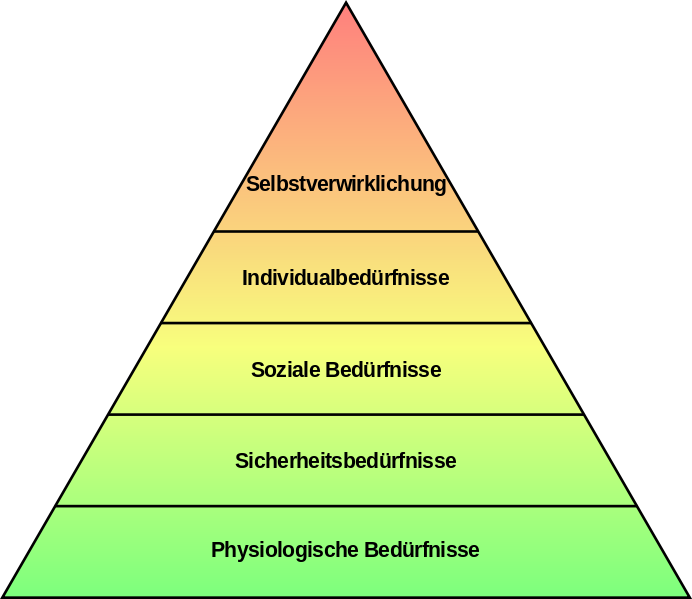
\includegraphics[scale=0.3]{pictures/lf02-pic/lf02-maslow.png}

Kritik an Maslows Theorie beginnt schon bei der Darstellungsform: die hierarchische Darstellung impliziert, dass ein einmal gestelltes Bedürfnis gestillt bleibt. Dies ist im Fall von Hunger offensichtlich falsch. Außerdem basiert Maslows Ansatz auf westlich-industriell sozialisiertem Statusdenken und einem Individualismus, der nicht selbstverständlich ist.

%%% Ende: Mitarbeitermotivation
%%%%%%%%%%%%%%%%%%%%%%%%%%%%%%%%%%%%%%%%%%%%%%%%%%%%%%%%%%%%%%%%%%%%%%%%%%%%%%%%

%%% Anfang: Führungsstile
\subsection{Führungsstile}

Im folgenden Abschnitt werden drei Führungsstile beschrieben. Zum ersten der autoritäre Führungsstil, zweitens der kooperative Führungsstil und drittens der Laissez-fair Führungsstil.

%%% Anfang: Führungsstile > Autoritär
\subsubsection{Autoritärer Führungsstil}
\begin{itemize}
	\item Die Mitarbeiter bei Entscheidungen nicht mitbestimmen lassen, sondern Entscheidungsprozesse alleine vollziehen
	\item Wichtige Aufgaben alleine übernehmen
	\item Die Mitarbeiter stark kontrollieren
	\item Die Fähigkeiten der Mitarbeiter stets als \ql gering\qr\ einschätzen
	\item Den Mitarbeitern wenig Freiraum überlassen
	\item Alleine die Verantwortung tragen
\end{itemize}

%%% Anfang: Führungsstile > Kooperativ
\subsubsection{Kooperativer Führungsstil}
\begin{itemize}
	\item Entscheidungen werden durch eine Mitarbeitergruppe getroffen und der Vorgesetzte tritt nur als Koordinator nach innen und außen auf
	\item Viele Aufgaben werden auf die Mitarbeiter übertragen
	\item Die Mitarbeiter werden bei den Arbeitsaufgaben wenig kontrolliert
	\item Die Fähigkeiten der Mitarbeiter werden wertgeschätzt und gefördert
	\item Den Mitarbeitern wird viel Freiraum gewährt
	\item Der Vorgesetzte trägt die Verantwortung gemeinsam mit den Mitarbeitern
\end{itemize}

%%% Anfang: Führungsstile > Laissez-faire
\subsubsection{Laissez-faire Führungsstil}
\begin{itemize}
	\item Entscheidungen werden den Mitarbeitern überlassen
	\item Alle Aufgaben werden auf die Mitarbeiter übertragen
	\item Die Mitarbeiter werden bei ihren Arbeitsaufgaben nicht kontrolliert
	\item Den Mitarbeitern wird nahezu grenzenloser Freiraum gelassen
	\item Der Vorgesetzt weist die Verantwortung von sich und überträgt diese auf die Mitarbeiter
	\item \ql gar kein Führungsstil\qr
\end{itemize}

%%% Ende: Führungsstile
%%%%%%%%%%%%%%%%%%%%%%%%%%%%%%%%%%%%%%%%%%%%%%%%%%%%%%%%%%%%%%%%%%%%%%%%%%%%%%%%

%%% Anfang: Berufsbildungsgesetz
\subsection{Berufsbildungsgesetz}

%%% Anfang: Berufsbildungsgesetz > Ausbildung
\subsubsection{Berufsausbildungsgesetz}

%%% Ende: Berufsbildungsgesetz
%%%%%%%%%%%%%%%%%%%%%%%%%%%%%%%%%%%%%%%%%%%%%%%%%%%%%%%%%%%%%%%%%%%%%%%%%%%%%%%%

%%% Anfang: Rechte und Plfichten
\subsection{Rechte und Pflichten von Auszubildenden}

%%% Ende: Rechte und Plfichten
%%%%%%%%%%%%%%%%%%%%%%%%%%%%%%%%%%%%%%%%%%%%%%%%%%%%%%%%%%%%%%%%%%%%%%%%%%%%%%%%